%%%%%%%%%%%%%%%%%%%%%%%%%%%%%% -*- Mode: Latex -*- %%%%%%%%%%%%%%%%%%%%%%%%%%%%
%% 12-17.tex --  Tech report on RAs
%% Author          : Philip Johnson
%% Created On      : Mon Sep 23 11:52:28 2002
%% Last Modified By: Philip Johnson
%% Last Modified On: Mon Jun 14 12:41:23 2010
%%%%%%%%%%%%%%%%%%%%%%%%%%%%%%%%%%%%%%%%%%%%%%%%%%%%%%%%%%%%%%%%%%%%%%%%%%%%%%%
%%   Copyright (C) 2009 Philip Johnson
%%%%%%%%%%%%%%%%%%%%%%%%%%%%%%%%%%%%%%%%%%%%%%%%%%%%%%%%%%%%%%%%%%%%%%%%%%%%%%%
%% 

\documentclass[]{article}
\usepackage{graphicx}
\usepackage{cite}
\usepackage{url}
\usepackage{enumitem}
\usepackage{times}
\usepackage[margin=1in]{geometry}

% uncomment the % away on next line to produce the final camera-ready version
% and uncomment the \thispagestyle{empty} following \maketitle
%\pagestyle{empty}
\begin{document}

%\onecolumn
%\setlength{\parindent}{0cm}


\title{{\bf Looking under the lamppost for useful software analytics}} 

\author{Philip M. Johnson\\
        Collaborative Software Development Laboratory\\
        Department of Information and Computer Sciences\\
        University of Hawai`i at M\=anoa\\
        Honolulu, HI 96822\\
        johnson@hawaii.edu\\
}


\maketitle

\thispagestyle{empty}


\setlength{\parskip}{3pt plus 1pt minus 1pt} 

\section{Introduction}
Noam Chomsky once said, {\em ``Science is a bit like the joke about the drunk who is looking under a lamppost for a key that he has lost on the other side of the street, because that's where the light is. It has no other choice.'' \cite{Barsky98}} For over 15 years, researchers at the Collaborative Software Development Laboratory at the University of Hawaii have looked for analytics that aid in understanding and improving the process and products of software development, and we believe Chomsky's scientific lamppost provides a useful metaphor for understanding both our efforts and those of other researchers in this area.

When it comes to analytics regarding software development processes and products, we claim
that ``looking under the lamppost'' refers to ``collecting and analyzing metrics that are easy
to obtain with little social, political, or developmental impact.''  In other words, the
easier an analytic is to collect,  and the less controversial it is to use, the more
limited its usefulness and generality.  For example, the data contained in a configuration
management repository is easy to collect and the intrinsically public nature of the
repository means that few developers will object to its analysis, but the
resulting analytics are intrinsically constrained by the very narrow slice of development
activity captured by this analytic. Conversely, the original version of the
Personal Software Process can yield extremely rich and impactful analytics, but with the
cost of significant overhead on developers along with significant social and political
implications for the analytics themselves.

We believe this tradeoff to be an essential characteristic of analytics for software
development processes and products, and that there is unlikely to be a technological
silver bullet that provides rich analytics without social and political implications.  To
justify this belief, we would like to briefly overview our findings from our search for
useful information about software development processes and products.

\section{It is better to light a candle: The Personal Software Process}

Our research on analytics for software processes and products began in 1996 when we
started using and evaluating the Personal Software Process (PSP) as described in Watts
Humphrey's ``A Discipline for Software Engineering'' \cite{Humphrey95}. This book was
innovative in several dimensions: it showed how organizational software process analytics
could be adapted to individual developers, it showed how these analytics could be used to
drive improvement, and it presented the practices in an incremental fashion amenable to
academic and professional adoption.

\begin{figure}[!tb]
\centering
\includegraphics[width=0.95\columnwidth]{defects.eps}
\caption{Sample Defect Recording Log. In the PSP, even compiler (syntax) errors are recorded.}
\label{fig:defect-log}
\end{figure}
 
This book's version of the PSP uses simple spreadsheets, manual data collection, and
manual analysis. The effort required to collect and manage this data is substantial: in
one version of the PSP, developers must fill out 12 separate forms, including a project
plan summary, a time recording log, a defect recording log, a process improvement
proposal, a size estimation template, a time estimation template, a design checklist, and
a code checklist. These forms typically yield over 500 distinct values that must be
manually calculated by the developer.  Interestingly, Humphrey actively embraced the
manual nature of the PSP, writing on page 217 that {\em ``It would be nice to have a tool
  to automatically gather the PSP data. Because judgement is involved in most personal
  process data, no such tool exists or is likely in the near future''}.  More
fundamentally, Humphrey viewed his predefined PSP processes as a
bootstrapping method: in Chapter 13, ``Defining the Software Process'', he exhorts
developers to modify the forms and procedures presented earlier in order to address their
specific circumstances and needs. That chapter presents a form developed by the author for
his personal use and labelled PSP7, five versions higher than the final predefined version prescribed
by the book (PSP 2.1).

From the perspective of our metaphor, we view this original version of the PSP as
``lighting a candle'' rather than looking under the lamppost because the approach promotes
custom, situationally-specific analytics. The manual nature of the PSP makes its analytics
fragile, in the same way that a candle flame is easy to extinguish.  But the manual nature
of the PSP also makes its analytics flexible: just as a candle enables its holder to
navigate in the darkness, the PSP enables and encourages its users to search for the
analytics best suited to their needs.  To make this clear, consider a developer who
suspects that the number of interruptions she experiences each morning directly impacts on
her productivity.  The PSP provides both explicit encouragement to explore this analytic,
the techniques with which to make a sound, evidence-based conclusion, and a relatively low cost
means to do so.  

Unfortunately, after using and teaching the predefined PSP processes for two years, we
began to suspect that the manual nature of the PSP created the potential for significant
data quality problems, and we designed an empirical study that 
checked over 30,000 data values generated by classroom use of the PSP
\cite{csdl-98-11}. We found that the manual nature of the PSP could sometimes lead to
incorrect process conclusions even though the overall error rate was very low---less than
5\%.  To address this problem, we embarked upon a new research project called Project
LEAP, and in retrospect, unwittingly compromised one of the best features of the PSP.

\section{Project LEAP: From candle to campfire} 

Project LEAP (Lightweight, Empirical, Anti-measurement dysfunction, and Portable software
process measurement) attempted to address the data quality problems we encountered with the manual
PSP through the development of a toolkit to automate and normalize data analysis
\cite{csdl-99-08}.  While the developer still entered most data by hand, the
toolkit automated subsequent PSP analyses and in some cases provided alternative
analyses (such as various forms of regression) not explored in the PSP.  It provided a
``lightweight'' approach by not prescribing the sequence of development activities 
(unlike the PSP). It attempted to avoid measurement dysfunction by enabling
developers to control their data files, by maintaining data about only one developer's
activities, and by not referencing developer names in the data files. Finally, LEAP data
was intended to be portable: a source of personal process data that the developer could
keep with them as they moved from project to project and organization to organization.
Figure \ref{fig:leap} illustrates one of the toolkit components, which supports time
estimation based upon personal historical data and selection of a regression analysis.

\begin{figure}[!tb]
\centering
\includegraphics[width=0.50\columnwidth]{planword.eps}
\caption{The time estimation toolkit component in Project LEAP.}
\label{fig:leap}
\end{figure}

Returning to our metaphor, Project LEAP replaces the PSP candle with a
``campfire''.  The introduction of higher level tool support metaphorically increases the
light by improving data quality and lowering the amount of manual analysis.  On the other
hand, unlike a candle, whose light can be moved around according to the interests
of the holder, a campfire is stationary: participants must come to it.  By introducing
automation, Project LEAP makes certain analytics easy to collect but others
disproportionately difficult.  Consider our hypothetical developer who suspects that
interruptions are impacting on her productivity: she would now be expected to design and
implement a new Leap toolkit component as opposed to a simple spreadsheet form.  

The LEAP toolkit was actively developed from 1997 to 2001, and used in
both classroom and industrial settings.  Industrial developers commented that they were
attracted to the fact that the toolkit offered much of the analytics associated with the
PSP without dictating the development process.  In 2001, the Agile Manifesto
\cite{AgileManifesto} was published, defining a name and set of principles that appeared
to stand in direct opposition to the PSP's commitment to process definition, adherence,
and high-overhead data collection and analysis. Instead, the agile community developed
relatively simple, low-overhead metrics such as velocity and burn-down.

After several years of using the LEAP toolkit, we came to agree with Humphrey that the PSP
approach could never be fully automated and would inevitably require a significant amount
of manual data entry.  We also came to agree with the Agile community that such overhead
frequently introduced excessive overhead into development without providing enough return
on investment, particularly when each project was sufficiently different from previous as
to render historical data inappropriate for comparison.

Our next project, however, departed from the conventional wisdom of both camps. Unlike the
PSP/TSP community, we would abandon any pretense of supporting PSP analyses.  Unlike the
agile community, we would continue to embrace extensive measurement and analysis.  The
research question was simple to state: what kinds of useful software analytics could be
obtained if both collection and analysis were ``free''?  Answering this question became
the mission of a decade-long research project called Hackystat.

\section{Hackystat:  The harsh glare of operating room lights}

As users of both the manual PSP as well as the LEAP toolkit, we were personally aware of
the overhead on development created by such data collection, even though there was
significant evidence for downstream benefits in the form of better planning and reduced
defects. The conventional wisdom, as prescribed by methodologies such as GQM
\cite{Basili94gqm}, is to define high-level goals first and then figure out the data
collection and analysis necessary to achieve them.  In the Hackystat research project
\cite{csdl2-02-07}, we chose to work in the opposite direction: we first focused on
developing ways to collect software process and product data with little to no overhead to
developers, and then explored what high-level software engineering goals could be
supported by analyses on this data. Hackystat implements a service-oriented architecture,
where sensors attached to development tools gather process and product data and send it
off to a server which can be queried by other services to build higher level analyses. 

Some of the important design features of Hackystat include:
\begin{itemize}
\item {\em Client as well as server-side data collection.}  Modern software development
  typically includes activities undertaken by individual developers on their local
  workstation as well as server (or cloud)-based activities. From the start, we developed
  instrumentation for client-side tools such as editors, build tools, test tools, as well
  as server-side tools such as configuration management repositories, build servers, etc.
\item {\em Unobtrusive data collection.}  One of the most frustrating aspects of manual data
  collection is the ``do some work, then interrupt your work to record what you worked on''
  loop. An important requirement for Hackystat was to make data collection as unobtrusive
  as possible: you should not notice that data is being collected, and the system should
  not make assumptions about network availability. For example, Hackystat client-side
  instrumentation locally caches any data collected while a developer is working
  offline, then sends the data to the Hackystat data repository once the developer
  reconnects. 
\item {\em Fine-grained data collection.}  By instrumenting client-side tools, we could
  collect data on a minute-by-minute or even second-by-second basis. For example, one type
  of data collection possible in Hackystat is called ``Buffer transition'', where a data
  instance is collected each time the developer changes the active buffer from one file to
  another.  We could track the developer as they edited a method, constructed a test case
  for that method, then invoked the test, yielding insight into test-driven development as
  it occurs ``in the real world''.
\item {\em Both personal and group-based development.}  In addition to tracking ``personal''
  development data, developers can define projects and shared artifacts to represent group
  work.  We could track the interplay between developers as they edited the same file. 
\end{itemize}

During the past ten years, we have discovered significant technical strengths as well as
significant political and social weaknesses in this approach.  Technically, Hackystat has
led to a broad variety of innovations, including the development of a toolkit for defining
and visualizing software project ``telemetry'' \cite{csdl2-04-11}, support for high
performance computing software development \cite{csdl2-04-22}, a method for prioritizing
what software development artifacts to inspect \cite{csdl2-05-01}, an operational
definition for Test-Driven Development \cite{csdl2-09-01}, an approach to software process
discovery \cite{csdl2-10-09}, and a mechanism called the ``Software ICU'' for assessing
the health of an individual project both alone and in relation to other projects
\cite{csdl2-09-02}.  Figure \ref{fig:icu} shows an image from this last Hackystat-based system.

\begin{figure}[!tb]
\centering
\includegraphics[width=1.0\columnwidth]{portfolio-2008.eps}
\caption{A software intensive care unit display, based on Hackystat.}
\label{fig:icu}
\end{figure}


In addition to discovering the analytic possibilities of this technology, we
also discovered significant social and political problems.  First, the unobtrusive nature of
data collection, which we viewed as a feature, was to some developers a bug: they did not
want to install instrumentation into their environment that would collect data regarding
their activities without telling them about it.  Second, the client-side, fine-grained
data collection can create discord within a development group: one
user referred to the Software ICU as ``hacky-stalk'', complaining about the
transparency it provided about each member's working style.  Third,
the client-side, fine-grained data providing the most compelling analytics about
development was simultaneously the largest obstacle to industrial adoption of Hackystat
technologies: developers repeatedly informed us that they were not comfortable with
management access to such data, despite management promises to use it appropriately. Robert
Austin provides much more details on this phenomena and its typical outcome of
``measurement dysfunction'' \cite{Austin96}.

To better understand these problems, it is helpful to take a closer look at the Software
ICU.  As shown on the left side of Figure \ref{fig:icu}, the Software ICU collects and
displays structural metrics about software artifacts, such as coverage, complexity,
coupling, and churn, and the Software ICU colors their most recently observed values and
their trends over time with red, yellow, or green to indicate their ``health''.  Another
structural metric is size, which the Software ICU displays for informational purposes but
presents in white (because the analysis has no way of characterizing current size or size
trends over time as ``healthy'' or ``unhealthy''.)  The Software ICU displays these values
for a portfolio of projects, allowing comparison of project data.  In general, collection,
analysis, and public presentation of the values to the left of the (white) Size data is
not controversial.

It is on the right side of the Software ICU interface where things get interesting, as
this side presents four indicators of ``health'' based upon aggregations of individual
developer behavior: DevTime, Commit, Build, and Test.  DevTime provides an estimate of how
much time each developer spends in their IDE working on each file associated with the
project; Commit measures how often each developer commits to the repository (and how many
lines of code are committed each time); Build measures how many times each developer
builds the system (and whether the build is successful); and Test measures how often each
developer invokes the test suite on the system (and whether the tests ran successfully).
In the Software ICU, clicking on any of the sparklines results in a drilldown to a more
detailed perspective. For example, clicking on the DevTime sparkline generates a
visualization showing individual DevTime trends for each developer.

While our research provides evidence that such a representation of individual developer
behavior makes some uncomfortable, it is also necessary if one is to provide certain kinds
of insight.  As a simple example, an aphorism of agile software development is ``build
early and often'', and the Software ICU can actually measure the extent to which
developers adhere to this principle.  

A more sophisticated application of developer behavior data occurs in the Hackystat-based
Zorro system, which can automatically determine the extent to which developers use
test-first design methods (popularly known as the ``red/green/refactor'' cycle).  Such an
analysis requires a very fine-grained, second-by-second analysis of developer behavior, as
illustrated in Figure \ref{fig:zorro}.

\begin{figure}[!tb]
\centering
\includegraphics[width=0.50\columnwidth, angle=270]{zorro.png.eps}
\caption{Recognizing Test-Driven Design development.}
\label{fig:zorro}
\end{figure}

Returning to our metaphor, Hackystat provides the equivalent of high intensity operating
room lights for software analytics. The approach provides the potential for abundant
illumination and deep insight, but these benefits often cannot be achieved without
procedures some might view as invasive.  Furthermore, the Hackystat philosophy of
automated collection would make it exceedingly difficult for our hypothetical
developer who suspects that interruptions are impacting on her productivity.  To fit 
the philosophy, she would have to design and implement some combination of hardware and
software to detect the presence of an interruption at her door and send data about its
start and end times to Hackystat for further analysis.

\section{The state of practice: back under the lamppost}

In the past few years, services for software product analytics have become popular, with
offerings from DevCreek, Ohloh, Atlassian, CAST, Parasoft, McCabe, Coverity, Sonar, and
others. The analytics for all of these services are typically built from one or more of
three basic sources: a configuration management system, a build system, and a defect
tracking system.  Figure \ref{fig:sonar} shows a display from Sonar for the SpringSource
project, which is representative for services of this type.

\begin{figure}[!tb]
\centering
\includegraphics[width=0.50\columnwidth, angle=90]{sonar-dashboard.eps}
\caption{The Sonar dashboard display, showing a collection of product metrics.}
\label{fig:sonar}
\end{figure}

These systems have two significant strengths.  First, data collection is entirely
automated and the data is already available; the service simply applies analytic
techniques (coverage, complexity, security, etc) to the data and provides a nice user
interface for the results. As the data is automatically gathered from a repository, the
overhead to developers and managers is low. Second, the data is generally
uncontroversial, in that it focuses on characteristics of the product and
not on the developer behaviors that produced these characteristics.

In our experience, these systems correspond best to the metaphor of ``looking under the
lamppost because that's where the light is''.  The systems are optimized for ease of
installation and integration, but the result is rather limited illumination of software
processes and products.  For example, our hypothetical developer who suspects that
interruptions are affecting her productivity is entirely out of luck: the approach simply
does not support such behavioral, client-side data collection and analysis. As a second
example, none of them could offer insight into the use of developer practices such as TDD.

\section{Conclusions and future directions}

Figure \ref{fig:axis} summarizes our experiences by illustrating three
basic trade-offs in the design of analytics for software process
and products.   The first trade-off is degree of automation, and what level of overhead is
incurred by developers and management to obtain the analytics.  The second trade-off is the barrier
to adoption incurred by the technique or technology, which could be social or political in
nature, and at its worst could lead to measurement dysfunction, undermining the
analytic entirely. The third trade-off, represented by the size of the circle in the figure, is the
level of generality of the technique or technology: how broad or narrow is the range of
analytics that can be developed while adhering to the essential characteristics of the
technique or technology? 

\begin{figure}[!tb]
\centering
\includegraphics[width=0.50\columnwidth, angle=90]{axis.pptx.eps}
\caption{A three dimensional classification for software analytics approaches, including 
  automation, adoption barriers, and breadth of possible analytics supported by the
  approach (indicated by the size of the circle).}
\label{fig:axis}
\end{figure}

As can be seen, Hackystat, PSP, and modern product analytic technologies like Sonar occupy
three distinct quadrants of the simple classification scheme presented in Figure
\ref{fig:axis}. The figure also shows how Agile measurements (such as velocity, burn-down,
and burn-up) fit into the fourth quadrant.  In addition, the figure present example analytics
for PSP, Hackystat, and Agile that would be difficult to implement by techniques or
technologies associated with the other quadrants.

After many years of exploring different approaches to analytics for software process and
products, we have concluded that the field is not converging on a single best approach,
nor that the very latest approaches are intrinsically better than prior ones.  Instead, we
find that the community has been exploring the space of trade-offs between expressiveness,
simplicity, and social acceptability.  

Consideration of these approaches also suggests two fruitful directions for future
research and practice.  First, a hybrid approach that mixes the best of automated
collection and analysis with carefully chosen, high impact manual data entry by developers
has the potential to substantially increase the impact of the analytics with acceptable
overhead to developers.  Second, modern approaches to privacy could assuage some developer
fears regarding behavioral data collection and analysis.  Consider a cloud-based,
independent, and privacy-oriented analytics repository, where developers could maintain
complete control over their data and whether to provide management access.  Just as
companies establish privacy mechanisms to encourage whistleblowers to come forward,
companies could decide that the benefits of insightful software analytics warrant
provisions to enable developers increased control. 

\section{Acknowledgements}

These findings result from the hard work of CSDL researchers since 1995 including:
Joy Agustin,  
Robert Brewer,
Joe Dane, 
Anne Disney, 
Jennifer Geis, 
Austin Ito, 
Aaron Kagawa,  
Honging Kou, 
Christoph Lofi, 
Carleton Moore, 
Mike Paulding, 
Dan Port,
Julie Sakuda,
Pavel Senin,
James Wang,
Cedric Zhang, and
Shaoxuan Zhang.

We also gratefully acknowledge the National Science Foundation, a primary sponsor of this
research through grants 9403475, 9804010, and 0234568.

All CSDL software is developed using open source licensing.  For more details on the
research and access to the software, please see http://csdl.ics.hawaii.edu.

\bibliographystyle{plain}
\bibliography{csdl-trs,psp,hackystat,12-11}
\end{document}
